\documentclass[a0,portrait]{a0poster}
%\usepackage{alltt}
\usepackage{color}
\usepackage{times}
\usepackage{a0poster}
\usepackage{graphicx}
\usepackage[utf8]{inputenc} % ÆØÅ pakken
\usepackage[T1]{fontenc}


%%%%%%%%%%%%%%%%%%%%%%%%%%%%%%%%%%%%%%%%%%%%%%%%%%%%%%%%%%%%%%%%%%%%%%%%%%%%%


\begin{document}

\title{Centralized State Estimation of Distributed Maritime} % Line one of the title
\titletwo{Autonomous Surface Oceanographers} % Line two of the title.
\author{Rasmus L. Christensen, Federik Juul, Nick \O stergaard, Tudor Muresan, Attila Fodor}
\address{Section for Control and Automation, Department of Electronic Systmes, Aalborg University, Denmark$^\dagger$}
\email{\{ralch,nickoe,fjuul,tudor,attila\}@es.aau.dk}

\makeheader

%% Column 1
\begin{center}
\col{
\paragraph{Introduction}
With the growing interest for cruise ships to sail close to shore in and around Greenland, better sea charts are highly needed. As Greenland have in excess of 30000 kilometer of shore line, measuring this manually is a both time consuming but also expensive task. A way to deal with this, could be to use a mothership with smaller drones 
\paragraph{Problem}
Is it possible to estimate the states of a ship using a centralized control strategy and a 9.6kbps radio link?
\paragraph{Path Planner}
Some text about the path planning software goes here, and it will be good. Remember some pictures! 
}
%% Column 2
\col{ 
\paragraph{Theory}
Some theory describing our problem and what theories we've been using!
\paragraph{State estimation}
Some text about the Kalman filter goes here - this will be used to go crazy! \cite{sorensen}
\paragraph{Simulation verification}
Once the vehicle have been tested, the actual measurements can be included here. 
\begin{figure} % Figure input
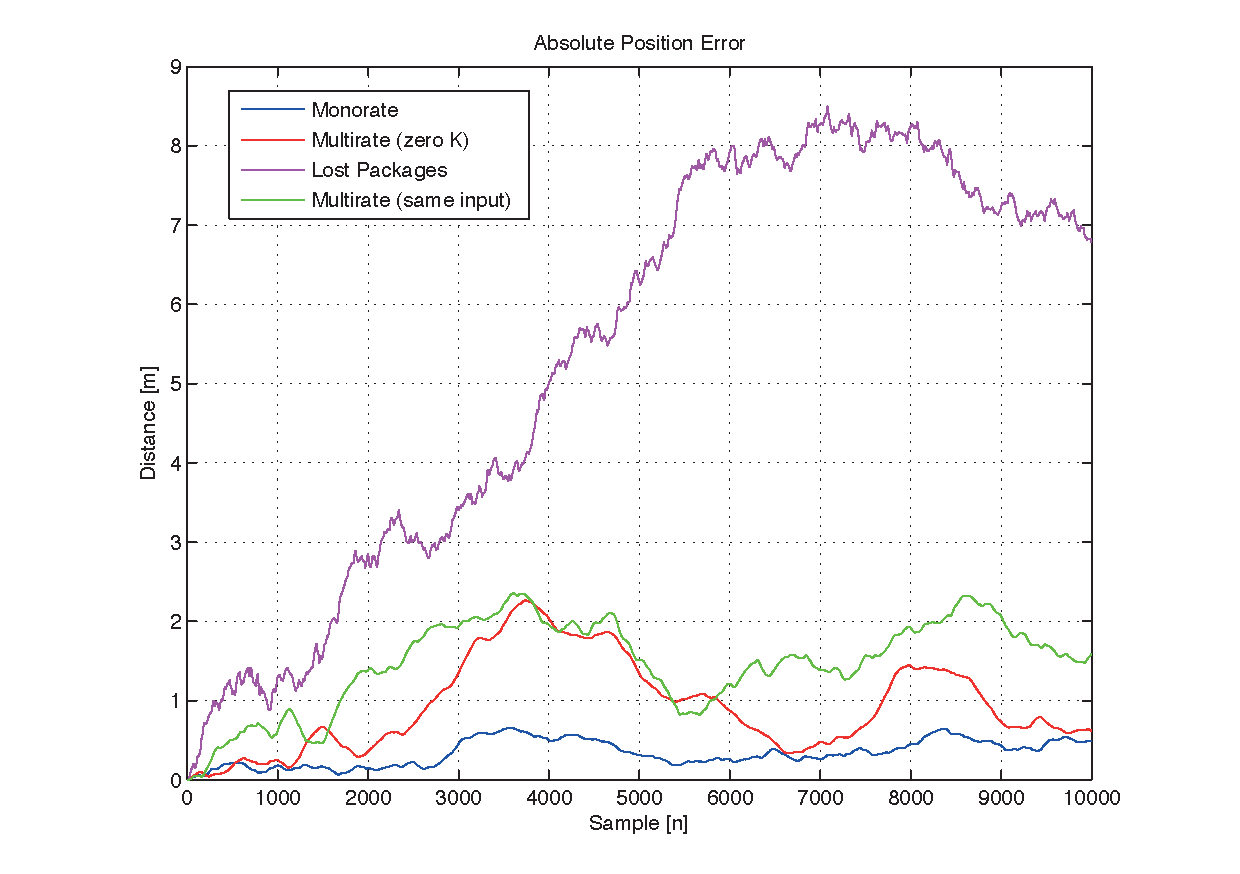
\includegraphics[size=\textwidth]{img/10percent}
  \caption{Simulation of the system with a packet loss rate of 10 percent}
\label{fig:trends}
\end{figure}
}
%% Column 3
\col{
\paragraph{Results}
Results on lost packages. 
\paragraph{Further results}
Something else?
\paragraph{Conclusion and extensions}
We can from this conclude that there is a problem.
\paragraph{Acknowledgements} We would like to thank DD-Plast in Randers for their support during the production of the ship.

\references
\bibliography{litterature}
}
\end{center}


\makefooter

\end{document}





